\begin{frame}{Teacher}
    \textbf{Esten Høyland Leonardsen}
    \begin{itemize}
        \item Master's degree in Informatics: Programming and Networks
        \item PhD in Psychology, deep learning applied to neuroimaging data
        \item Experience as a data scientist and programmer from the industry and various start-ups
        \item Post-doc at the center for Cognitive psychology, Neuroscience and Neuropsychology
        \item Chief Scientific Officer at baba.vision
        \item Interests: Deep learning, explainable artificial intelligence, mental health, neuroimaging
    \end{itemize}
\end{frame}

\begin{frame}{Students}
    \textbf{What I want to know about you}
    \begin{itemize}
        \item What's your name?
        \item What department/section are you from?
        \item What's your research project about?
        \item Do you have experience with machine learning and/or programming?
        \item What do you hope to learn from this course? (e.g. specific applications in your research, a theoretical understanding of machine learning, following and contributing to the public discourse, a future job in data science, ...)
    \end{itemize}
\end{frame}

\begin{frame}{About the course}
    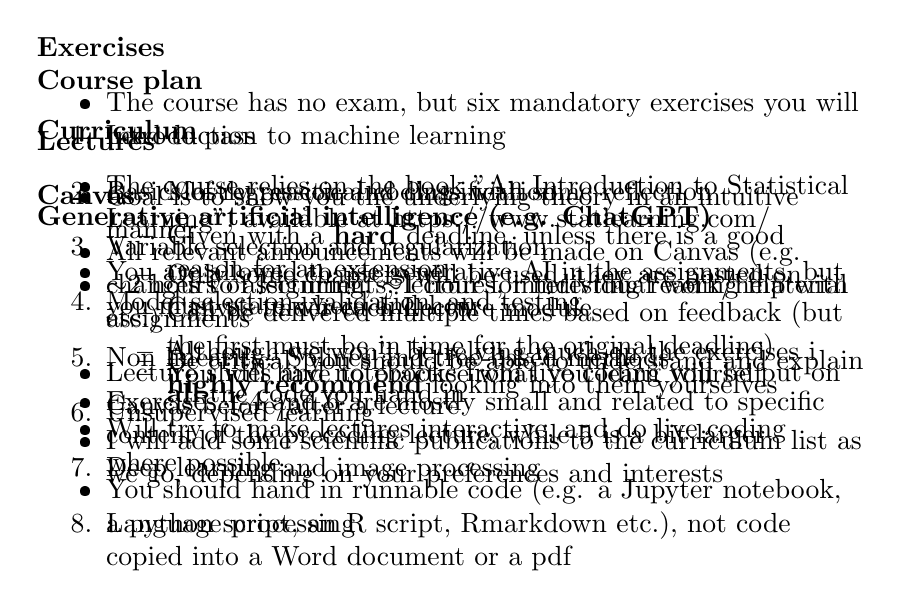
\begin{tikzpicture}
    \visible<1>{
        \node[text width=10.5cm] at (0, 0) {
            \textbf{Canvas}
            \begin{itemize}
                \item All relevant announcements will be made on Canvas (e.g. changes to assignments, lectures, interesting reading material etc.)
                \item Lecture slides and notebooks from live coding will be put on Canvas before/after a lecture
            \end{itemize}
        };
    }
    \visible<2>{
        \node[text width=10.5cm] at (0, 0) {
            \textbf{Curriculum}
            \begin{itemize}
                \item The course relies on the book "An Introduction to Statistical Learning", available at \url{https://www.statlearning.com/}
                \begin{itemize}
                    \item Only some chapters will be used, they are posted on Canvas under each Lecture module
                    \item Although we won't be relying much on the exercises i \textbf{highly recommend} looking into them yourselves
                \end{itemize}
                \item I will add some scientific publications to the curriculum list as we go, depending on your preferences and interests
            \end{itemize}
        };
    }
    \visible<3>{
        \node[text width=10.5cm] at (0, 0) {
            \textbf{Exercises}
            \begin{itemize}
                \item The course has no exam, but six mandatory exercises you will need to pass
                \begin{itemize}
                    \item Mostly practical coding, with some reflection
                    \item Given with a \textbf{hard} deadline, unless there is a good reason for an extension
                    \item Can be delivered multiple times based on feedback (but the first must be in time for the original deadline)
                \end{itemize}
                \item Exercises 1-4 and 6 are mostly small and related to specific content of the preceding lecture, while 5 is a bit larger
                \item You should hand in runnable code (e.g. a Jupyter notebook, a python script, an R script, Rmarkdown etc.), not code copied into a Word document or a pdf
            \end{itemize}
        };
    }
    \visible<4>{
        \node[text width=10.5cm] at (0, 0) {
            \textbf{Generative artificial intelligence (e.g. ChatGPT)}
            \begin{itemize}
                \item You are allowed to use generative AI in the assignments, but you must state where and how
                \begin{itemize}
                    \item Be critical, you should be able to understand and explain \textbf{all} the code you hand in
                \end{itemize}
            \end{itemize}
        };
    }
    \visible<5>{
        \node[text width=10.5cm] at (0, 0) {
            \textbf{Lectures}
            \begin{itemize}
                \item Goal is to show you the underlying theory in an intuitive manner
                \item $\sim$2 hours of lecturing, $\sim$1 hour for individual work/help with assignments
                \begin{itemize}
                    \item You will have to practice what you learn yourself
                \end{itemize}
                \item Will try to make lectures interactive, and do live coding where possible
            \end{itemize}
        };
    }
    \visible<6>{
        \node[text width=10.5cm] at (0, 0) {
            \textbf{Course plan}
            \begin{enumerate}
                \item Introduction to machine learning
                \item Basics of regression and classification
                \item Variable selection and regularization
                \item Model selection, validation, and testing
                \item Non linearity: Splines and tree-based methods
                \item Unsupervised learning
                \item Deep learning and image processing
                \item Language processing
            \end{enumerate}
        };
    }
    \end{tikzpicture}
\end{frame}
